\documentclass[10pt,a4paper]{article}
\usepackage[T1]{fontenc}
\usepackage{graphicx}
\usepackage{float}
\usepackage{fancyhdr}
\begin{document}
	\noindent 1. Given the dataset below. You can give any meaning to the numbers in the table. Nonetheless, our focus is to compare ANOVA with the regression with dummy variables. First, import the table into R as a data frame manually, after which you can use \textit{aov()} to run ANOVA and \textit{lm()} to run regression. Please try to figure out how to assign dummy coding/variables to different groups, and check the similarity between the results from two methods.
	
	\begin{figure}[H]
		\centering
		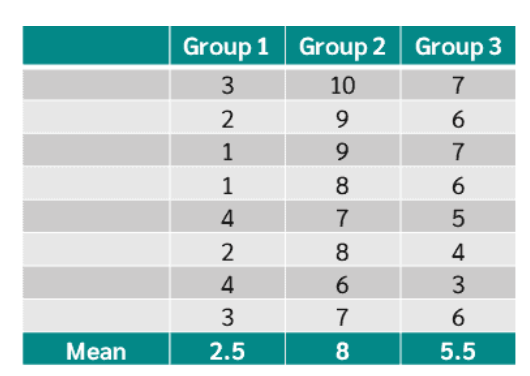
\includegraphics[width=0.7\textwidth]{F:/PsychoStatisticia/Course/12-week Course/统计学提高班/Week6/data_1_ANOVA.png}
		\caption{Data for question 2}
	\end{figure}
	
	\noindent 2. Recall the example we mentioned in last lecture. We have \textit{salary} as the criterion variable (Y) in our model, and use 2 dummy variables $X_1, X_2$ to code 3 levels of \textit{job titles}. Additionally, we have \textit{years of work} as a continuous predictor. Finally, assume we have the model below:
	
	\begin{equation}
		y=\beta_0+\beta_1X_1+\beta_2X_2+\beta_3year+\beta_4X_1year+\beta_5X_2year+\epsilon
	\end{equation}
	
	Try to interpret all $\beta$s above in the model by making use of the knowledge you learned in the lecture.
\end{document}